%bNEWSystemTest
%test
\section{System test}
This section covers the test of the system, prior to conducting the experiment for the project. 

\subsection{Method of Test for Gyroscopes}
The Shimmer3 devices were calibrated using the built in function of Shimmer Sensing’s program, Consensys, to ensure the devices would work as expected \cite{ShimmerSensing2016}.

%til test af gyro/accel kan vi gøre som paul foreslog og filme personen imens de drejer rundt eller noget, hvor vi kan synkronisere film med gyro/accel målinger og se at der sker udsving på samme tidspunkt som personen drejer/bevæger sig. Det kan self ikke være med i rapporten men vi kan vise det til eksamen. 


\subsection{Method of Test for Force Sensitive Resistors}
The FSRs were tested by placing a 1kg weight covering a surface area of 1$cm^{2}$ applied in the middle of both types of FSRs. This was done to test if any of the sensors were broken or deviated from the values of the other FSRs. %mean result of the test.

%retfærdigøre at vi brugere sensore der "kun" kan måle så lidt tryk til at måle under folk som vejer +50 kg. Sikkert noget med at simon har sat modstande i systemet som øger sensorernes måling af tryk påvirkning. 

\subsection{Test  Results for Force Sensitive Resistors}
A weight of 1kg were applied to each FSR in order from FSR channel 1 to 6. The weight was applied for approximately five seconds to each FSR in the middle of the sensor area. Results of the FSR test is shown in \figref{fig:FSRTestPlot1kg}.

\begin{figure}[H]
	\includegraphics[width=.7\textwidth]{figures/FSRTestPlot1kg}
	\caption{The result of the test of the six FSRs.}
	\label{fig:FSRTestPlot1kg}  %<--remember LABEL!
\end{figure}

As it can be seen from the results none of the sensors were broken, however FSR number 3 (FSR3), located at the heel of the right foot, returned a lower resistance when applied a 1kg weight compared to the other FSRs.

%Tell the truth.
%The authors learned too late in the work period that one of the FSRs were returning resistance varying from the other FSRs. This was not anticipated and no replacement had been ordered. However, the authors hope/judge/evaluate that the FSR will not affect the data processing the calculations of Centre of Pressure (COP) too much.

%tell the lie
%During continuous testing of the system during development the authors experienced damage to one of the FSRs, and are at this point in the work, unable to obtain a replacement. However, as this project is mainly to function as a proof of concept work, the authors determine that one sensor should not have too much of an effect.

%tell the something-in-between
This could prove a problem if data were to be compared between individual FSRs, however the output for each FSR sensors was used for estimation of a point for the subjects COP, which were be used to compare COP between subjects. Thus, the FSR3 measurement would not have an effect as long as FSR3 had the same deviance for every subject. 

A later analysis of acquired data from the subjects performances showed that the readings FSR3 had small variance when compared to readings from the other FSRs. \Figref{fig:FSRpostTest} shows the mnaximum recorded values for each FSR during kata performance for all subjects. Here FSR3 recordings have little variance from other FSRs. 

\begin{figure}[H]
	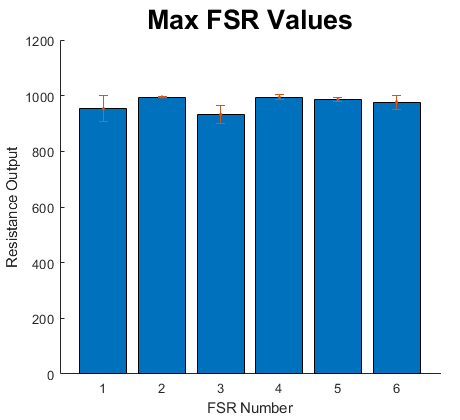
\includegraphics[width=.7\textwidth]{figures/FSRValues}
	\caption{Barchart of maximum FSR recordings for all kata repetitions for all subjects.}
	\label{fig:FSRpostTest}  %<--remember LABEL!
\end{figure}



\subsection{System Test}
The system as a whole was tested with a walk sequence. The sequence involved periods of no movement, movement by walking and turning and a light jump to mark the beginning and end of the sequence. The test walk sequence was as follows:
\vspace{-0.6cm}
\begin{itemize}
	\item 5 second pause
	\vspace{-0.3cm}
	\item Light jump
	\vspace{-0.3cm}
	\item 5 second pause
	\vspace{-0.3cm}
	\item Walk five steps
	\vspace{-0.3cm}
	\item 180 degree turn
	\vspace{-0.3cm}
	\item Walk five steps
	\vspace{-0.3cm}
	\item 5 second pause
	\vspace{-0.3cm}
	\item Light jump
	\vspace{-0.3cm}
	\item 5 second pause
\end{itemize}
\vspace{-0.4cm}
%Test walk sequence: Wait 3 sec. light jump. wait 1 sec. walk 5 steps. 180 turn. walk 5 steps. 90 turn right. wait. 90 turn right. wait. quick 180. wait quick 180. wait 1. light jump. wait 3 sec. 
Following the system test the acquired data was qualitatively evaluated to ensure everything worked as intended. 

\subsection{Results for System Test}
%Everything was fine. maybe.
Result of the system test as a whole were successful, despite lower readings from FSR3. Acquired data was plotted for each FSR channel, so the recorded output could be viewed alongside a video recording of the test walk sequence. At each step FSRs were reacting and returning values consistent with what would be expected when pressure was either applied to or removed from the sensors. 
It was concluded that, as the lower resistance returned from FSR3 was consistent for all data collection, the \textit{"error"} would be present in each data set and therefore would not have any effect on comparison between subjects. Later analysis of data showed this to be correct.

%not necessary 
%A problem occurred with the FSR 406 placed under the heel of the subject during the system test . When weight was applied to the sensor it would measure the highest possible force the sensor can measure, and no useful data could be collected from the sensor. It was evaluated why this happened and discovered that because the FSR 406 covers a larger area and were placed at the heel it would be affected by more force when a subject stood on it. As the distribution of pressure is higher at the heel compared to anywhere else under the foot while standing, it makes sense that the FSR 406 would be overloaded \cite{Hessert2005}. To account for this, the FSR 402 placed at the lateral side of the feet where switched with the FSR 406 at the heel. As the FSR 402 covers a smaller area they would not be overloaded as easily as the FSR 406. As a result the FSR 406 is now placed at the lateral side of the eminence of the sole, and one FSR 402 is placed at the heel. The new placement of FSR sensors can be seen in \figref{fig:soleSensorPlacement}.
%With the new placement of the FSR’s the system functions as intended and is ready for the experiment. 
